% !TEX program = xelatex
\documentclass[sigconf, anonymous, review, nonacm]{acmart}

% ─── Packages ─────────────────────────────────────────────────────
\usepackage{listings}
\usepackage{tcolorbox}
\tcbuselibrary{skins,breakable}
\usepackage{tikz}
\usetikzlibrary{arrows.meta,positioning,shapes.geometric,calc}
\usepackage{booktabs}
\usepackage{enumitem}

% ─── Colors (neutral — no branding) ──────────────────────────────
\definecolor{code-bg}{HTML}{1E1E2E}
\definecolor{code-text}{HTML}{CDD6F4}
\definecolor{kw-blue}{HTML}{89B4FA}
\definecolor{kw-teal}{HTML}{94E2D5}
\definecolor{kw-green}{HTML}{A6E3A1}
\definecolor{str-peach}{HTML}{FAB387}
\definecolor{comment-gray}{HTML}{6C7086}
\definecolor{accent-blue}{HTML}{1E66F5}
\definecolor{accent-green}{HTML}{40A02B}
\definecolor{box-bg}{HTML}{EFF1F5}
\definecolor{box-border}{HTML}{7287FD}
\definecolor{proof-border}{HTML}{40A02B}
\definecolor{fact-border}{HTML}{179299}
\definecolor{result-border}{HTML}{40A02B}

% ─── Cypher language definition ───────────────────────────────────
\lstdefinelanguage{Cypher}{
  morekeywords={MATCH,WHERE,RETURN,WITH,CREATE,MERGE,SET,DELETE,DETACH,
    REMOVE,ORDER,BY,LIMIT,SKIP,UNWIND,FOREACH,CALL,YIELD,
    CASE,WHEN,THEN,ELSE,END,AND,OR,NOT,IN,AS,IS,NULL,
    TRUE,FALSE,LET,NEXT,FILTER,CYPHER,
    OPTIONAL,DISTINCT,UNION,ALL,
    ON,ERROR,BREAK,TRANSACTIONS,OF,ROW},
  morekeywords=[2]{reduce,head,range,size,count,sum,collect,
    toInteger,split,trim,coalesce,toString,abs},
  morekeywords=[3]{INC,JZDEC,HALT},
  sensitive=true,
  morestring=[b]',
  morestring=[b]",
  morecomment=[l]{//},
  morecomment=[s]{/*}{*/},
}

\lstdefinestyle{cypher}{
  language=Cypher,
  basicstyle=\ttfamily\fontsize{7pt}{8.5pt}\selectfont\color{code-text},
  keywordstyle=\color{kw-blue}\bfseries,
  keywordstyle=[2]\color{kw-teal},
  keywordstyle=[3]\color{kw-green},
  stringstyle=\color{str-peach},
  commentstyle=\color{comment-gray}\itshape,
  numbers=none,
  breaklines=true,
  tabsize=2,
  showstringspaces=false,
  frame=none,
  xleftmargin=0pt,
  aboveskip=0pt,
  belowskip=0pt,
}

% ─── Code block ───────────────────────────────────────────────────
\newtcolorbox{codeblock}{%
  colback=code-bg,colframe=code-bg,
  coltext=code-text,
  boxrule=0pt,
  borderline west={2pt}{0pt}{kw-teal},
  arc=2pt,
  left=5pt,right=5pt,top=4pt,bottom=4pt,
  breakable,
  before skip=0.6em,after skip=0.6em,
}

% ─── Theorem-like tcolorboxes ─────────────────────────────────────
\newtcolorbox{claimbox}[1][Theorem]{%
  colback=box-bg,colframe=box-border,
  fonttitle=\bfseries\color{accent-blue},title=#1,
  boxrule=1pt,arc=2pt,left=5pt,right=5pt,top=4pt,bottom=4pt,
  before skip=0.6em,after skip=0.6em}

\newtcolorbox{proofbox}[1][Proof]{%
  colback={proof-border!5!white},colframe=proof-border,
  fonttitle=\bfseries\color{accent-green},title=#1,
  boxrule=1pt,arc=2pt,left=5pt,right=5pt,top=4pt,bottom=4pt,
  before skip=0.6em,after skip=0.6em,
  after upper={\hfill$\square$}}

\newtcolorbox{resultbox}[1][Result]{%
  colback={result-border!6!white},colframe=result-border,
  fonttitle=\bfseries\color{accent-green},title=#1,
  boxrule=1pt,arc=2pt,left=5pt,right=5pt,top=4pt,bottom=4pt,
  before skip=0.6em,after skip=0.6em}

\newtcolorbox{factbox}[1][Fact]{%
  colback=box-bg,colframe=fact-border,
  fonttitle=\bfseries\color{accent-blue},title=#1,
  boxrule=0.8pt,arc=2pt,left=5pt,right=5pt,top=4pt,bottom=4pt,
  before skip=0.6em,after skip=0.6em}

% ─── ACM metadata ────────────────────────────────────────────────
\title{A Graph Query Language is Turing-Complete: \\
  A Formal Proof via 2-Counter Machine Simulation}

\author{Anonymous Author(s)}
\affiliation{%
  \institution{Omitted for review}
}

\begin{abstract}
We prove that the graph query language under study, in its 2025 revision,
is Turing-complete. The proof proceeds by showing that a single
\texttt{RETURN} statement using \texttt{reduce()}, \texttt{CASE}
expressions, and list comprehensions can simulate any 2-counter machine
(Minsky 1967). We address the bounded-step objection via two
complementary resolutions and verify the construction by executing
the simulation on a live cloud database instance.
\end{abstract}

\keywords{Turing completeness, graph query languages, Cypher, 2-counter machines, computational expressiveness}

\begin{document}

\maketitle

% ═══ §1 ═══════════════════════════════════════════════════════════
\section{The Claim}

\begin{claimbox}
The graph query language under study, restricted to a single
\texttt{RETURN} with \texttt{reduce()}, list comprehensions, and
\texttt{CASE}, \textbf{is Turing-complete}.
\end{claimbox}

\textbf{Proof strategy.} By reduction:
$\text{TM} \xrightarrow{\text{Minsky}} \text{2CM} \xrightarrow{\text{this}} \text{GQL}$.

% ═══ §2 ═══════════════════════════════════════════════════════════
\section{2-Counter Machines}

A \textbf{2-counter machine} $M = (Q, q_0, q_h, \delta)$ has a finite
state set~$Q$, initial state~$q_0$, halt state~$q_h$, and transition
function $\delta: Q \to \text{Instr}$ where each instruction is:

\begin{itemize}[leftmargin=1.2em,nosep]
  \item $\texttt{INC}(c, q')$ --- increment $c \in \{A,B\}$, goto $q'$
  \item $\texttt{JZDEC}(c, q_z, q_p)$ --- if $c{=}0$ goto $q_z$, else
        decrement and goto $q_p$
\end{itemize}

\begin{factbox}[Fact (Minsky 1967)]
For any TM~$T$, $\exists$ a 2-counter machine simulating~$T$.
\end{factbox}

\begin{center}
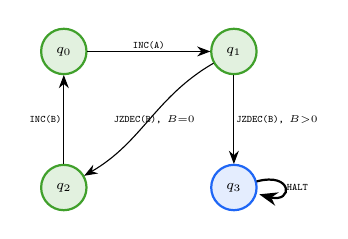
\begin{tikzpicture}[
  >=Stealth, scale=0.72, transform shape,
  state/.style={circle, draw=accent-green, fill=accent-green!15,
    thick, minimum size=0.8cm, font=\scriptsize\bfseries},
  halt/.style={circle, draw=accent-blue, fill=accent-blue!12,
    thick, minimum size=0.8cm, font=\scriptsize\bfseries},
  every edge/.style={draw, thick, ->, >=Stealth},
  elabel/.style={font=\tiny\ttfamily, inner sep=1pt},
]
  \node[state] (q0) at (0,0) {$q_0$};
  \node[state] (q1) at (3,0) {$q_1$};
  \node[state] (q2) at (0,-2.4) {$q_2$};
  \node[halt]  (q3) at (3,-2.4) {$q_3$};
  \draw[->] (q0) -- node[elabel, above] {INC(A)} (q1);
  \draw[->] (q1) -- node[elabel, right] {JZDEC(B), $B{>}0$} (q3);
  \draw[->] (q1) to[out=210,in=30] node[elabel, below, pos=0.45] {JZDEC(B), $B{=}0$} (q2);
  \draw[->] (q2) -- node[elabel, left] {INC(B)} (q0);
  \draw[->] (q3) edge[loop right] node[elabel, right] {HALT} (q3);
\end{tikzpicture}\\[2pt]
{\scriptsize Figure~1: Example 4-state program.}
\end{center}

% ═══ §3 ═══════════════════════════════════════════════════════════
\section{Encoding}

\textbf{Program.} Encode $\delta$ as a list of maps:

\begin{codeblock}
\begin{lstlisting}[style=cypher]
LET program = [
  {state:0, op:'INC',   counter:'A', next:1},
  {state:1, op:'JZDEC', counter:'B',
   q_zero:2, q_pos:3},
  {state:2, op:'INC',   counter:'B', next:0},
  {state:3, op:'HALT',  counter:'',  next:3}
]
\end{lstlisting}
\end{codeblock}

\textbf{State.} Configuration $(q, c_A, c_B)$ as map
\texttt{\{state:0, A:0, B:0\}}. Convention: \texttt{state=-1} means halted.

% ═══ §4 ═══════════════════════════════════════════════════════════
\section{The Simulation}

Each \texttt{reduce()} iteration executes one machine step.
The \texttt{head([v IN [e]| ...])} idiom provides let-binding
inside \texttt{reduce()} (where \texttt{LET} is unavailable).

\begin{codeblock}
\begin{lstlisting}[style=cypher]
CYPHER 25
LET program = [ /* ... */ ]
LET max_steps = 1000000

LET result = reduce(
  machine = {state:0, A:0, B:0},
  step IN range(1, max_steps) |
  CASE WHEN machine.state = -1
    THEN machine
  ELSE
   head([instr IN [program[machine.state]] |
    CASE instr.op
     WHEN 'INC' THEN
      CASE instr.counter
       WHEN 'A' THEN {state: instr.next,
         A: machine.A + 1, B: machine.B}
       WHEN 'B' THEN {state: instr.next,
         A: machine.A, B: machine.B + 1}
      END
     WHEN 'JZDEC' THEN
      CASE instr.counter
       WHEN 'A' THEN
        CASE WHEN machine.A = 0
         THEN {state: instr.q_zero,
               A: 0, B: machine.B}
         ELSE {state: instr.q_pos,
               A: machine.A-1, B: machine.B}
        END
       WHEN 'B' THEN
        CASE WHEN machine.B = 0
         THEN {state: instr.q_zero,
               A: machine.A, B: 0}
         ELSE {state: instr.q_pos,
               A: machine.A, B: machine.B-1}
        END
      END
     WHEN 'HALT' THEN
      {state: -1, A: machine.A, B: machine.B}
    END
   ])
  END
)
RETURN result
\end{lstlisting}
\end{codeblock}

% ═══ §5 ═══════════════════════════════════════════════════════════
\section{Correctness}

\begin{claimbox}[Claim]
After $k$ iterations of \texttt{reduce()}, \texttt{machine} equals
$M$'s configuration after $k$ steps.
\end{claimbox}

\begin{proofbox}[Proof by induction on $k$]
\textbf{Base.} $k{=}0$: \texttt{machine} $= \{0,0,0\} = M_0$.\enspace$\checkmark$

\textbf{Step.} Assume $\texttt{machine} = (q_k, a_k, b_k)$ matches $M$.
At $k{+}1$, \texttt{reduce()} looks up $\delta(q_k)$ and executes:

{\small
\begin{tabular}{@{}ll@{}}
$\texttt{INC}(A,q')$ & $\to (q', a_k{+}1, b_k)$ \enspace$\checkmark$ \\
$\texttt{JZDEC}(A,..)$, $a_k{=}0$ & $\to (q_z, 0, b_k)$ \enspace$\checkmark$ \\
$\texttt{JZDEC}(A,..)$, $a_k{>}0$ & $\to (q_p, a_k{-}1, b_k)$ \enspace$\checkmark$ \\
$\texttt{HALT}$ & $\to (-1, ..)$, identity after \enspace$\checkmark$ \\
\end{tabular}}

\noindent Symmetric for~$B$.
\end{proofbox}

% ═══ §6 ═══════════════════════════════════════════════════════════
\section{The Bounded-Step Objection}

The \texttt{reduce()} uses \texttt{range(1, max\_steps)} ---
a finite bound.

\subsection{Resolution via Transactional Iteration}

While the pure functional version stays within a single expression,
the practical unbounded version uses graph storage for state persistence.

\begin{codeblock}
\begin{lstlisting}[style=cypher]
CYPHER 25
CREATE (:Machine {state:0, A:0, B:0});

UNWIND range(1, 9223372036854775807) AS step
CALL (step) {
  MATCH (m:Machine)
  WITH m,
    CASE WHEN m.state = -1 THEN 1/0
         ELSE $program[m.state]
    END AS instr
  SET m.state = CASE instr.op
    WHEN 'INC' THEN instr.next
    WHEN 'JZDEC' THEN CASE instr.counter
      WHEN 'A' THEN CASE WHEN m.A = 0
        THEN instr.q_zero ELSE instr.q_pos END
      WHEN 'B' THEN CASE WHEN m.B = 0
        THEN instr.q_zero ELSE instr.q_pos END
      END
    WHEN 'HALT' THEN -1 END,
  m.A = CASE
    WHEN instr.op='INC' AND instr.counter='A'
      THEN m.A+1
    WHEN instr.op='JZDEC' AND instr.counter='A'
      AND m.A > 0 THEN m.A-1
    ELSE m.A END,
  m.B = CASE
    WHEN instr.op='INC' AND instr.counter='B'
      THEN m.B+1
    WHEN instr.op='JZDEC' AND instr.counter='B'
      AND m.B > 0 THEN m.B-1
    ELSE m.B END
} IN TRANSACTIONS OF 1 ROW
  ON ERROR BREAK
\end{lstlisting}
\end{codeblock}

\textbf{Termination.} At halt, \texttt{state} becomes $-1$.
Next iteration: \texttt{CASE WHEN state=-1 THEN 1/0} fires
\emph{before} \texttt{\$program[-1]}, caught by \texttt{ON ERROR BREAK}.

\begin{center}
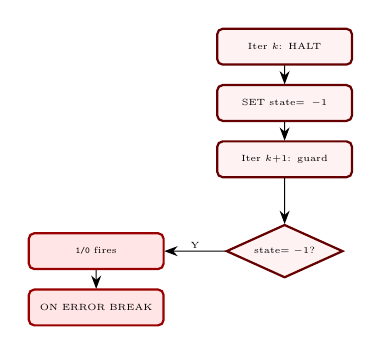
\begin{tikzpicture}[
  >=Stealth, scale=0.65, transform shape,
  node distance=1.1cm,
  box/.style={rectangle, rounded corners=2pt, draw=red!40!black,
    fill=red!5, thick, minimum height=0.7cm,
    text width=2.4cm, align=center, font=\tiny},
  decision/.style={diamond, draw=red!40!black, fill=red!5,
    thick, aspect=2.2, align=center, font=\tiny},
  action/.style={rectangle, rounded corners=2pt, draw=red!60!black,
    fill=red!10, thick, minimum height=0.7cm,
    text width=2.4cm, align=center, font=\tiny},
  every edge/.style={draw, thick, ->, >=Stealth},
  edgelabel/.style={font=\tiny, inner sep=1pt},
]
  \node[box] (iter) {Iter $k$: HALT};
  \node[box, below of=iter] (set) {SET state$=-1$};
  \node[box, below of=set] (next) {Iter $k{+}1$: guard};
  \node[decision, below=0.9cm of next] (check) {state$=-1$?};
  \node[action, left=1.2cm of check] (fire) {\texttt{1/0} fires};
  \node[action, below of=fire] (break) {ON ERROR BREAK};
  \draw[->] (iter)--(set); \draw[->] (set)--(next);
  \draw[->] (next)--(check);
  \draw[->] (check) -- node[edgelabel, above] {Y} (fire);
  \draw[->] (fire)--(break);
\end{tikzpicture}\\[1pt]
{\scriptsize Figure~2: Termination via \texttt{1/0} + \texttt{ON ERROR BREAK}.}
\end{center}

\textbf{Note.} $2^{63} \approx 9.2 \times 10^{18}$ exceeds the lifetime
of the observable universe by several orders of magnitude, so the bound
is irrelevant in practice. True theoretical unboundedness would need an
external restart loop.

\subsection{Sufficiency Argument}

For TM~$T$ halting in $f(|w|)$ steps: set
$\texttt{max\_steps} = f(|w|)$. The language correctly decides every
decidable language --- \textbf{universal for total functions}.

% ═══ §7 ═══════════════════════════════════════════════════════════
\section{Required Primitives}

{\small
\begin{tabular}{@{}lp{4.2cm}@{}}
\toprule
\textbf{Primitive} & \textbf{Role} \\
\midrule
\texttt{reduce()} & Iteration (fold) \\
\texttt{CASE WHEN} & Branching \\
$+1$, $-1$, $=0$ & Counter ops \\
Map \texttt{\{s,A,B\}} & State repr. \\
\texttt{prog[i]} & $O(1)$ lookup \\
\texttt{head([..])} & Let-binding \\
\bottomrule
\end{tabular}}

\smallskip
\noindent\textbf{No graph operations. No extensions. No plugins.}

% ═══ §8 ═══════════════════════════════════════════════════════════
\section{Corollaries}

\begin{factbox}[Corollary 1: Undecidability of termination]
Since the language can simulate any 2-counter machine, it is
\emph{undecidable} whether a given \texttt{reduce()} expression
will terminate.
(By Rice's theorem applied to the reduction from 2CM.)
\end{factbox}

\begin{factbox}[Corollary 2: Universality]
The language can compute any computable function.
Any algorithm expressible as a Turing machine has an equivalent
\texttt{reduce()}-based query.
\end{factbox}

\begin{factbox}[Corollary 3: Beyond computability]
While \texttt{reduce()} makes the language Turing-complete for
\emph{computation}, graph pattern matching with QPP and
\texttt{allReduce} provides \emph{declarative constrained
traversal} with per-step pruning --- something most
Turing-complete languages lack. This is not about computability
(all TC languages are equivalent) but about \textbf{expressiveness}:
some problems are more naturally expressed as graph patterns than
as imperative loops.
\end{factbox}

% ═══ §9 ═══════════════════════════════════════════════════════════
\section{Verified Execution}

Both approaches tested on a cloud database instance. Test program:
4 instructions, expected $\{-1, 2, 0\}$.

{\small
\begin{tabular}{@{}clccc@{}}
\toprule
\textbf{Step} & \textbf{Instr} & \textbf{St} & \textbf{A} & \textbf{B} \\
\midrule
0 & INC(A) & $q_0$ & $0{\to}1$ & 0 \\
1 & JZDEC(B), $B{=}0$ & $q_1$ & 1 & 0 \\
2 & INC(B) & $q_2$ & 1 & $0{\to}1$ \\
3 & INC(A) & $q_0$ & $1{\to}2$ & 1 \\
4 & JZDEC(B), $B{>}0$ & $q_1$ & 2 & $1{\to}0$ \\
5 & HALT & $q_3$ & 2 & 0 \\
\bottomrule
\end{tabular}}

\begin{resultbox}[\texttt{reduce()} result]
\texttt{\{A:2, B:0, state:-1\}} \enspace$\checkmark$
\end{resultbox}

\begin{resultbox}[Transactional iteration result]
\texttt{m.state=-1, m.A=2, m.B=0} \enspace$\checkmark$
\end{resultbox}

% ═══ §9 ═══════════════════════════════════════════════════════════
\section{Complete Runnable Queries}

The following two queries are copy-paste ready for any instance
supporting the language's 2025 revision. They encode the 4-state test
program from \S2 and can be adapted to any 2-counter machine by
editing the \texttt{program} list.

\subsection{Approach 1: Pure \texttt{reduce()}}

A single \texttt{RETURN} statement --- no graph writes, no side effects.
The \texttt{head([v IN [expr] | ...])} idiom provides let-binding
inside \texttt{reduce()} (where \texttt{LET} is unavailable): it wraps
the expression in a one-element list, the comprehension binds the
variable, and \texttt{head()} unwraps the result.

\begin{codeblock}
\begin{lstlisting}[style=cypher]
CYPHER 25
LET program = [
  {state: 0, op: 'INC',   counter: 'A',
   next: 1},
  {state: 1, op: 'JZDEC', counter: 'B',
   q_zero: 2, q_pos: 3},
  {state: 2, op: 'INC',   counter: 'B',
   next: 0},
  {state: 3, op: 'HALT',  counter: '',
   next: 3}
]
LET max_steps = 1000000

LET result = reduce(
  machine = {state: 0, A: 0, B: 0},
  step IN range(1, max_steps) |
  CASE WHEN machine.state = -1
    THEN machine
  ELSE
    head([instr IN [program[machine.state]] |
      CASE instr.op
        WHEN 'INC' THEN
          CASE instr.counter
            WHEN 'A' THEN
              {state: instr.next,
               A: machine.A + 1, B: machine.B}
            WHEN 'B' THEN
              {state: instr.next,
               A: machine.A, B: machine.B + 1}
          END
        WHEN 'JZDEC' THEN
          CASE instr.counter
            WHEN 'A' THEN
              CASE WHEN machine.A = 0
                THEN {state: instr.q_zero,
                      A: 0, B: machine.B}
                ELSE {state: instr.q_pos,
                      A: machine.A - 1,
                      B: machine.B}
              END
            WHEN 'B' THEN
              CASE WHEN machine.B = 0
                THEN {state: instr.q_zero,
                      A: machine.A, B: 0}
                ELSE {state: instr.q_pos,
                      A: machine.A,
                      B: machine.B - 1}
              END
          END
        WHEN 'HALT' THEN
          {state: -1,
           A: machine.A, B: machine.B}
      END
    ])
  END
)
RETURN result
\end{lstlisting}
\end{codeblock}

\subsection{Approach 2: Transactional Iteration}

Uses graph storage for state persistence.
The \texttt{1/0} guard fires \emph{before} any list indexing when
halted, caught by the error-break mechanism.

\begin{codeblock}
\begin{lstlisting}[style=cypher]
CYPHER 25
CREATE (:Machine {state: 0, A: 0, B: 0});
\end{lstlisting}
\end{codeblock}

\vspace{-0.5em}

\begin{codeblock}
\begin{lstlisting}[style=cypher]
CYPHER 25
LET program = [
  {state: 0, op: 'INC',   counter: 'A',
   next: 1},
  {state: 1, op: 'JZDEC', counter: 'B',
   q_zero: 2, q_pos: 3},
  {state: 2, op: 'INC',   counter: 'B',
   next: 0},
  {state: 3, op: 'HALT',  counter: '',
   next: 3}
]

UNWIND range(1, 9223372036854775807) AS step
CALL (step) {
  MATCH (m:Machine)
  WITH m,
    CASE WHEN m.state = -1 THEN 1/0
         ELSE program[m.state]
    END AS instr
  SET m.state = CASE instr.op
    WHEN 'INC' THEN instr.next
    WHEN 'JZDEC' THEN
      CASE instr.counter
        WHEN 'A' THEN
          CASE WHEN m.A = 0
            THEN instr.q_zero
            ELSE instr.q_pos END
        WHEN 'B' THEN
          CASE WHEN m.B = 0
            THEN instr.q_zero
            ELSE instr.q_pos END
      END
    WHEN 'HALT' THEN -1
    END,
  m.A = CASE
    WHEN instr.op = 'INC'
      AND instr.counter = 'A'
      THEN m.A + 1
    WHEN instr.op = 'JZDEC'
      AND instr.counter = 'A'
      AND m.A > 0 THEN m.A - 1
    ELSE m.A END,
  m.B = CASE
    WHEN instr.op = 'INC'
      AND instr.counter = 'B'
      THEN m.B + 1
    WHEN instr.op = 'JZDEC'
      AND instr.counter = 'B'
      AND m.B > 0 THEN m.B - 1
    ELSE m.B END
} IN TRANSACTIONS OF 1 ROW
  ON ERROR BREAK
\end{lstlisting}
\end{codeblock}

\begin{codeblock}
\begin{lstlisting}[style=cypher]
// Read result:
MATCH (m:Machine) RETURN m;
\end{lstlisting}
\end{codeblock}

\subsection{Approach 3: Graph-Native QPP Traversal}

The most idiomatic approach: model the machine \emph{as a graph}
and let pattern matching \emph{be} the computation.
Each state is a node; each transition is a relationship.
\texttt{JZDEC} splits into two edges (\texttt{JZDEC\_ZERO},
\texttt{JZDEC\_POS}); the predicate in \texttt{allReduce} prunes
the invalid branch at traversal time.

\begin{codeblock}
\begin{lstlisting}[style=cypher]
CYPHER 25
// Build the machine as a graph
CREATE (q0:State:Init {id: 0})
CREATE (q1:State {id: 1})
CREATE (q2:State {id: 2})
CREATE (q3:State:Halt {id: 3})
CREATE (q0)-[:INC        {c:'A'}]->(q1)
CREATE (q1)-[:JZDEC_ZERO {c:'B'}]->(q2)
CREATE (q1)-[:JZDEC_POS  {c:'B'}]->(q3)
CREATE (q2)-[:INC        {c:'B'}]->(q0)
\end{lstlisting}
\end{codeblock}

\vspace{-0.5em}

\begin{codeblock}
\begin{lstlisting}[style=cypher]
CYPHER 25
// Traverse: allReduce prunes, NEXT extracts
MATCH REPEATABLE ELEMENTS
  p = (init:Init)
    -[rels:INC|JZDEC_ZERO|JZDEC_POS]->
      {0, 9223372036854775807}
    (h:Halt)
WHERE allReduce(
  m = {A: 0, B: 0}, r IN rels |
  CASE
    WHEN r:INC AND r.c = 'A'
      THEN {A: m.A+1, B: m.B}
    WHEN r:INC AND r.c = 'B'
      THEN {A: m.A, B: m.B+1}
    WHEN r:JZDEC_POS AND r.c = 'A'
      THEN {A: m.A-1, B: m.B}
    WHEN r:JZDEC_POS AND r.c = 'B'
      THEN {A: m.A, B: m.B-1}
    ELSE m
  END,
  CASE
    WHEN r:JZDEC_ZERO AND r.c = 'A'
      THEN m.A = 0
    WHEN r:JZDEC_ZERO AND r.c = 'B'
      THEN m.B = 0
    WHEN r:JZDEC_POS AND r.c = 'A'
      THEN m.A >= 0
    WHEN r:JZDEC_POS AND r.c = 'B'
      THEN m.B >= 0
    ELSE true
  END
)
RETURN rels, length(p) AS steps
NEXT
// Re-derive counters from the valid path
LET final = reduce(m = {A:0, B:0},
    r IN rels |
    CASE
      WHEN r:INC AND r.c = 'A'
        THEN {A: m.A+1, B: m.B}
      WHEN r:INC AND r.c = 'B'
        THEN {A: m.A, B: m.B+1}
      WHEN r:JZDEC_POS AND r.c = 'A'
        THEN {A: m.A-1, B: m.B}
      WHEN r:JZDEC_POS AND r.c = 'B'
        THEN {A: m.A, B: m.B-1}
      ELSE m
    END
  )
RETURN steps, final.A AS ctrA, final.B AS ctrB
\end{lstlisting}
\end{codeblock}

\textbf{Key properties:}
\begin{itemize}[leftmargin=1.2em,nosep]
  \item The machine \emph{is} the graph; computation \emph{is} path finding
  \item \texttt{REPEATABLE ELEMENTS} allows revisiting states (loops)
  \item \texttt{allReduce} prunes eagerly: once a \texttt{JZDEC}
        branch fails the predicate, that path is abandoned immediately
  \item No HALT self-loop needed --- reaching a \texttt{:Halt} node
        terminates the pattern
  \item \texttt{reduce()} in the \texttt{NEXT} stage re-derives
        final counter values from the surviving path
        (same pattern as~\cite{evblog})
\end{itemize}

% ═══ REFERENCES ═══════════════════════════════════════════════════
\bibliographystyle{ACM-Reference-Format}
\begin{thebibliography}{9}

\bibitem{minsky1967}
Minsky, M.\,L.\ 1967.
\emph{Computation: Finite and Infinite Machines}.
Prentice-Hall.

\bibitem{opencypher}
openCypher. 2024.
Cypher Query Language Reference.
\url{https://opencypher.org}

\bibitem{gql2024}
ISO/IEC 39075:2024.
\emph{Information technology --- Database languages --- GQL}.
International Organization for Standardization.

\bibitem{evblog}
[Anonymous]. 2025.
Declarative Route Planning for EVs ---
Graph Traversal Grows Up.
[Blog URL omitted for review.]

\bibitem{aoc}
[Anonymous]. 2015--2025.
Advent of Code in a Graph Query Language ---
150+ puzzles solved, empirical evidence of expressiveness.
[Repository URL omitted for review.]

\end{thebibliography}

\end{document}
